\section{Novelty ? }


Dealing with rewards for kills and deaths was not straight forward due to the long lag period between an action that resulted in one of these events and the event occuring. To assign rewards to killing the opponent, the last action the agent took that dealt damage is recorded as a "last damaging action". When the opponent dies, a large reward is assigned to this "last damaging action". This is necessary to avoid assigning large rewards to actions that are irrelevant to the result of the opponent dying.
\begin{figure}
	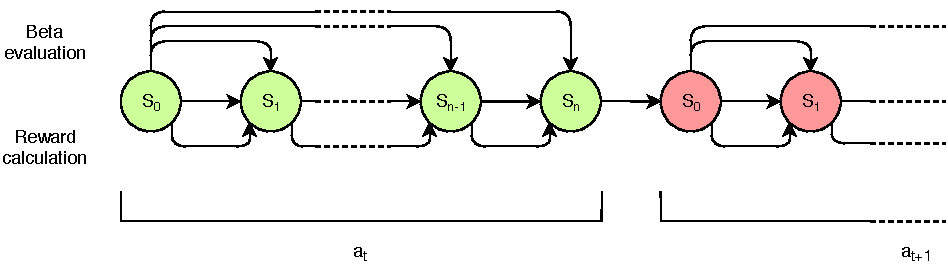
\includegraphics{stateevolution.pdf}
\end{figure}

Lastly, a finite length action history is tracked for the purposes of assigning negative rewards to deaths. When the agent dies, all actions in the action history are penalized, as the agent could have taken an action in this time frame that may have prevented its death but ultimately chose not to.An example of this is the agent being slightly off the edge of the stage and not choosing to jump back on. The action selected instead of jumping back on is then penalized.

